% -*-LaTeX-*-
\documentclass{sig-alternate-10pt}
\clubpenalty=10000
\widowpenalty = 10000

\usepackage{times,latexsym}
\usepackage[caption=false]{subfig}
\usepackage[sort]{cite}
\usepackage[hyphens]{url}
\usepackage{lastpage}
\usepackage{array, verbatim}
\usepackage{mdwlist}
\hyphenpenalty=5000
\tolerance=1000

\usepackage{multirow}

\newcommand\todo[1]{}

\setlength{\pdfpagewidth}{8.5in}
\setlength{\pdfpageheight}{11in}

\usepackage{ifpdf}
\usepackage{graphicx}
\graphicspath{{./figs2011/}}

\ifpdf
  \DeclareGraphicsExtensions{.pdf}
\else
  \DeclareGraphicsExtensions{.eps}
\fi
\twocolumn
\usepackage{mathtools}
\usepackage{alltt}
\usepackage{wasysym}
\usepackage{listings}
\usepackage{array}
%\usepackage{pdfcomment}
%\usepackage[rgb]{xcolor}

\renewcommand\floatpagefraction{.9}
\renewcommand\topfraction{.9}
\renewcommand\bottomfraction{.9}
\renewcommand\textfraction{.1}   
\setcounter{totalnumber}{50}
\setcounter{topnumber}{50}
\setcounter{bottomnumber}{50}

\newcommand{\enote}[2]{({\bf{#1:} \it{#2}})}
%\newcommand{\enote}[2]{}


\begin{document}

\title{Broadband Access in the US}
\author{
Zachary Bischof\\
Christopher Moran
}
  
\maketitle

%******************************************************************************
\begin{abstract}
 
Understanding the quality of Internet services that are available to customers is
import to government organizations surveying broadband availability in their 
country.

In this work, we study the quality (in terms of download throughput) of
broadband services available across the US. We used data provided by the FCC to
analyze trends in the quality of services available to customers in a region.
We compare this against census data, looking at how the quality of broadband
services relates to the median average income, finding that, in general,
regions with a higher median income have wider access to faster services.
However, using data collected by Ono, a BitTorrent extension, we find that
these services are not widely used, or at least fully utilized, in BitTorrent
traffic.

\end{abstract}

%******************************************************************************
\section{Problem Statement}
\label{sec:statement} 

In today's world, the Internet has become a crucial component of many aspects
of our society.  Aspects such as entertainment, education, finance, publishing,
shopping, and communication have all changed drastically in the past 10 years
due to the development and expansion of broadband Internet availability. In
some countries, Internet access is now considered a one of a citizen's rights.

Due to the broad implications of Internet access, many governments have begun
studying their network infrastructure, in order to verify that ISPs are
providing what they advertise, and that their citizens have satisfactory 
access to the Internet.  Of course, depending on the country, what is 
considered "satisfactory" is subjective.

The goal of this work is to provide a more detailed description of the quality
of broadband services in the US.  This includes the identification of other
factors, such as a region's median income, population, and household size.
Furthermore, we investigate what we actually see from a sample of BitTorrent
users.  



%******************************************************************************
\section{Prior Work}
\label{sec:prior-work}

In recent years, there has been a significant increase in the number of studies
attempting to degree of broadband Internet access, as well as the quality 
of those services.  To this end, the FCC of the US conducted a survey of ISPs
to see what services were available in regions across the US.  Their results
include the name of an ISP, their fastest available services, and the 
typical measured throughput for each zip code.  In this work, we examine this 
dataset and compare it with data collected by the US Census Bureau. The census
data includes information for each zip code, including the total population,
median income, and the average number of people per household.

Projects such as BISmark and their joint research with the FCC and SamKnows
focus on measuring characterizing ISP performance by distributing wireless
routers to users' homes, plugged directly into the modem. The focus of these
projects focus on measuring ISP performance, ensuring that what a customer
signs up for matches what the ISP actually provides.  However, in this work,
we attempt to identify other factors that determine the quality of services 
that are available to a customer in a particular region.
 

%******************************************************************************
\section{Approach}
\label{sec:approach} 

We begin by first joining the FCC's broadband map dataset, with the Census
Bureau's dataset at the zip code level. We examined both the typical download
speeds available in the region, as well as the advertised services.  Due to the
fact that a large number of counties across the US had much faster "typical"
speeds than "advertised" speeds, we excluded those results from the paper. 

After joining the two datasets, we checked for a correlation between a zip 
code's population and advertised speeds, as well as a zip code's median income
and advertised speeds.  The population of a zip code

%******************************************************************************
\section{Results}
\label{sec:results} 

\begin{table}
    \centering
    \small
    \begin{tabular}{ | l | l | l |}
    \hline
    \textbf{Tier} & \textbf{Lower} & \textbf{Upper} \\
    \textbf{Class} & \textbf{Threshold} & \textbf{Threshold} \\ \hline
    2 & 200 kbps & 768 kbps \\ \hline
    3 & 768 kbps & 1.5 Mbps \\ \hline
    4 & 1.5 Mbps & 3 Mbps \\ \hline
    5 & 3 Mbps & 6 Mbps \\ \hline
    6 & 6 Mbps & 10 Mbps \\ \hline
    7 & 10 Mbps & 25 Mbps \\ \hline
    8 & 25 Mbps & 50 Mbps \\ \hline
    9 & 50 Mbps & 100 Mbps\\ \hline
    10 & 100 Mbps & 1 Gbps\\ \hline
    11 & 1 Gbps & -- \\ \hline
    \end{tabular}
\caption{The bins used in the FCC's broadband map dataset 
for describing download throughput.
For example, class ``5'' corresponds to an ISP offering 
with a maximum download throughput between 3 Mbps and
6 Mbps.}
\label{table:service-classes}
\end{table}

\begin{figure*}
\centering
        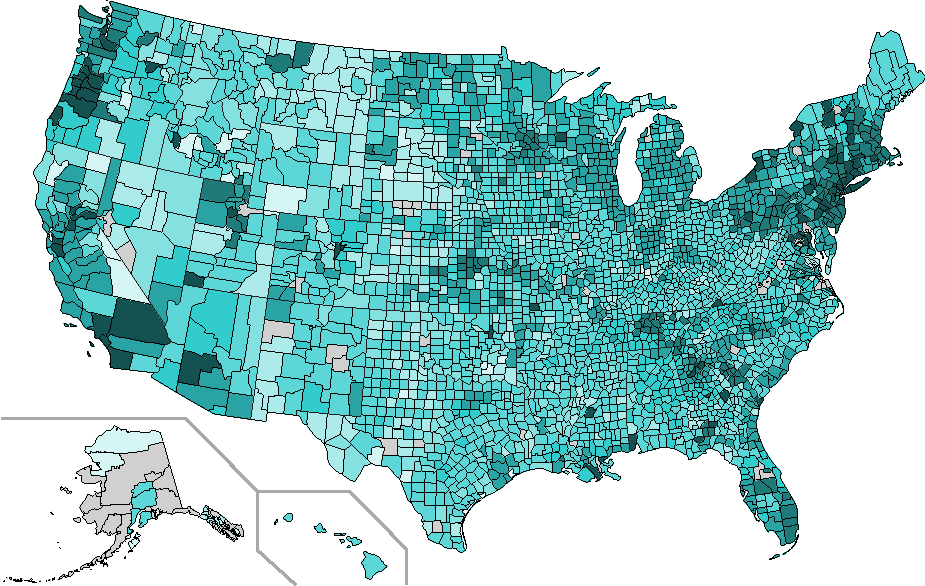
\includegraphics[width=0.9\linewidth]{figs/counties_maxDown.pdf}
  \caption{The maximum class of service that is available in a county, as
advertised by the ISP.  The
darker colors represent faster tiers of broadband service in terms of 
download throughput.}
  \label{fig:services-repMaxRepDown}
\end{figure*}

%\begin{figure*}
%\centering
%        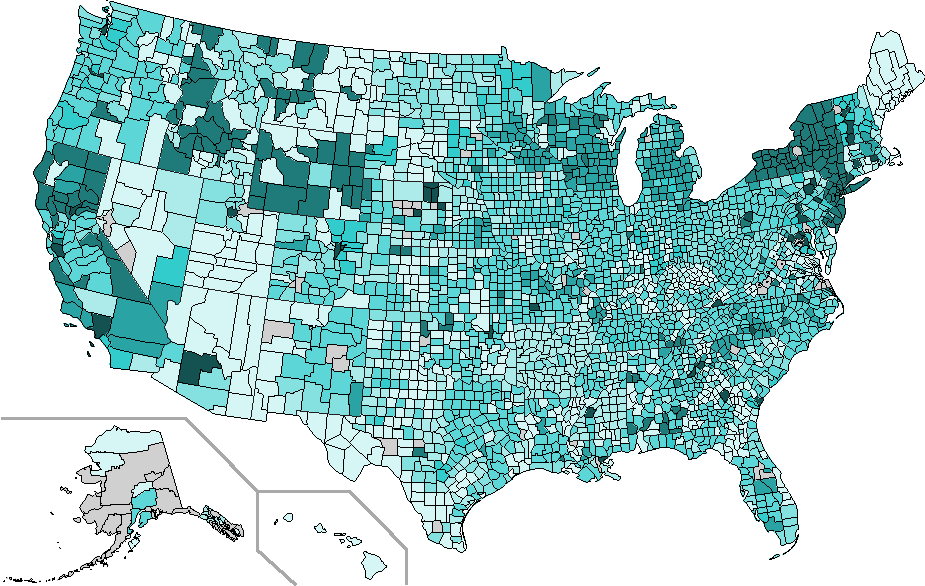
\includegraphics[width=0.9\linewidth]{figs/counties_typDown.pdf}
%  \caption{ The maximum typical download speed that is available in a
%county, reported by measurements in the study. Again, the darker
%colors represent faster tiers of broadband services. Many counties are 
%reported as having a significantly higher typical speed 
%than advertised speed (e.g. most of New York, northern California). }
%  \label{fig:services-repTypDown}
%\end{figure*}


\begin{figure}
\centering
        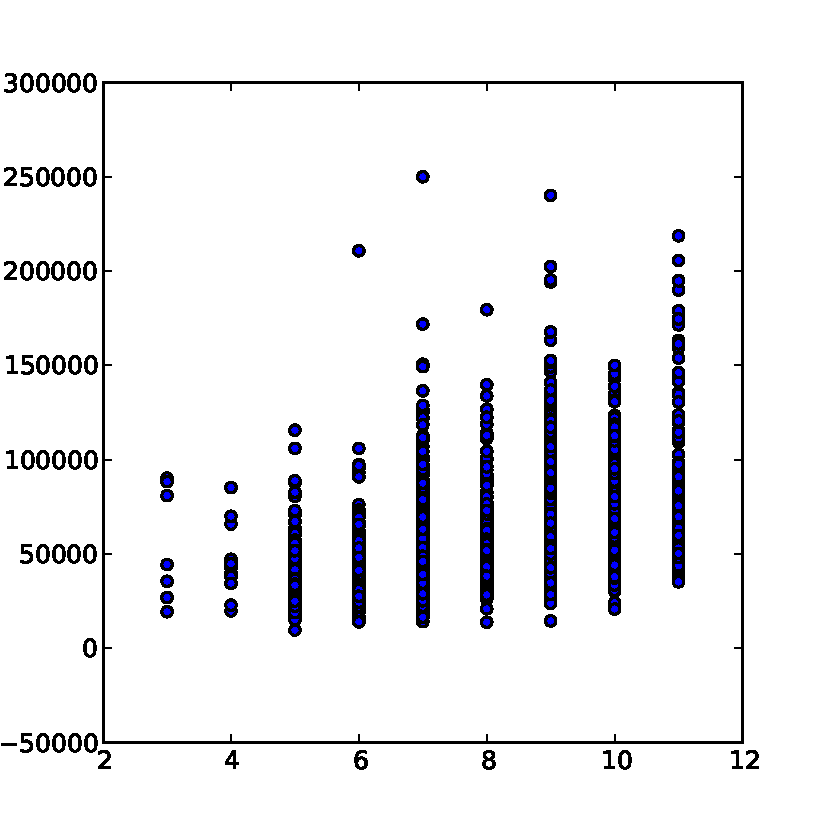
\includegraphics[width=0.9\linewidth]{figs/maxIncome_maxDown.pdf}
  \caption{The fastest service speed that is available 
in a particular zip code versus the median income for that
zip code.}
  \label{fig:services-incomeVsDown}
\end{figure}

\begin{figure}
\centering
        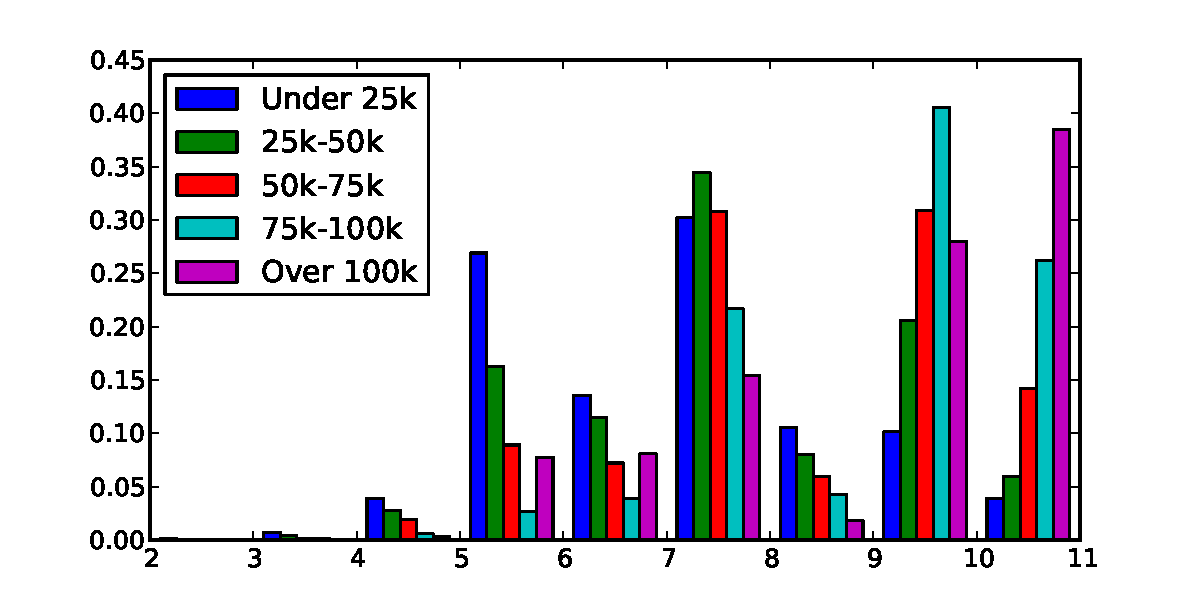
\includegraphics[width=0.9\linewidth]{figs/all_hist.pdf}
  \caption{The fraction of regions whose fastest available Internet
service falls into that level of service in terms of download throughput.
Regions are separated by the median income for that region.}
  \label{fig:services-hist}
\end{figure}

\begin{figure*}
\centering
        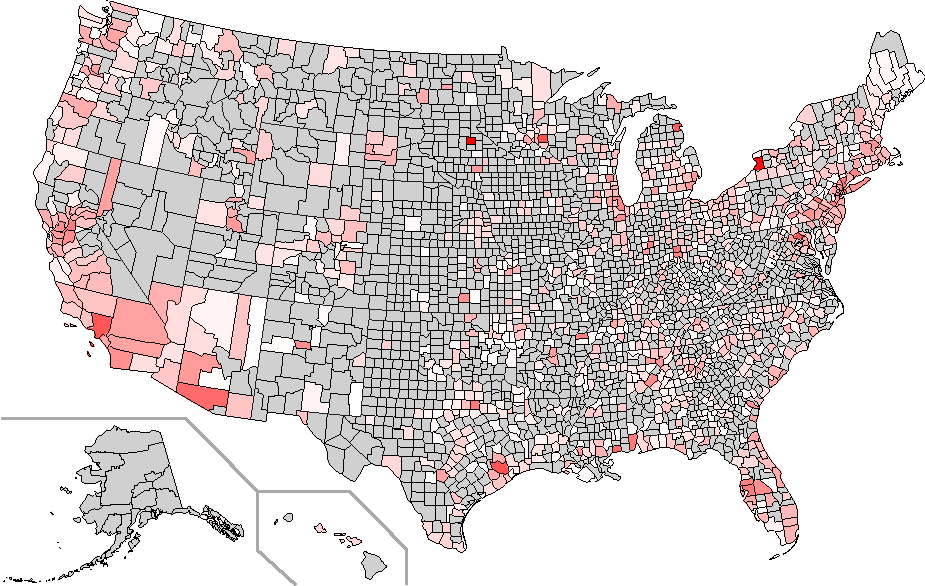
\includegraphics[width=0.9\linewidth]{figs/counties_btMaxDown.pdf}
  \caption{The maximum download bandwidth reported in counties across the 
US.  Counties colored gray did not have any sample points.  Red corresponds
to 100 Mbps while white corresponds to 100 kbps.}
  \label{fig:services-btMaxDown}
\end{figure*}

\begin{figure*}
\centering
        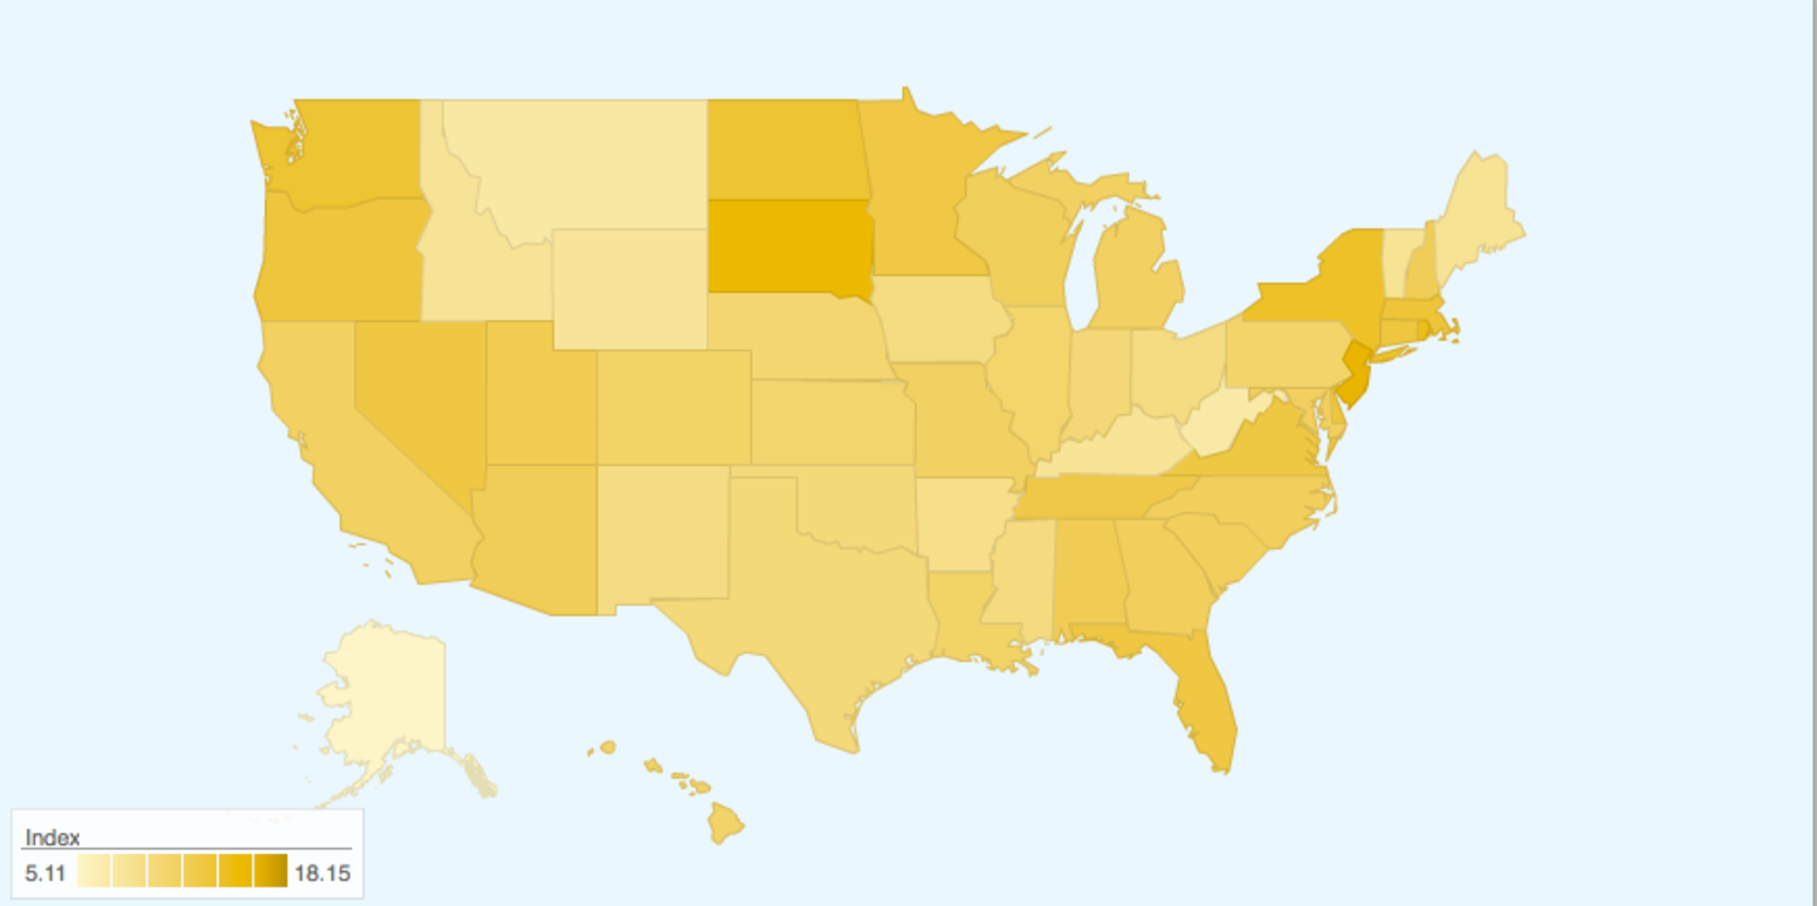
\includegraphics[width=0.9\linewidth]{figs/map.pdf}
  \caption{The netindex's map of the US, showing the average 
user download throughput from speedtest.net results.}
  \label{fig:services-net-index-map}
\end{figure*}

%******************************************************************************
\section{Future Work}
\label{sec:future-work} 

There are still many ways to aggregate and compare the datasets that we have
collected.  One aspect we'd be interested in seeing is the quality of services
that are available and commonly subscribed to in a focused geographic location.
In cities with areas of lower and higher median incomes, we plan to compare the
services available. For example, we could compare speeds in the north side,
south side, and suburbs of Chicago, as well as speeds in areas of low or high
population density both within and across cities (e.g. compare services in New
York City and Los Angeles).  

We also plan to conduct a longitudinal study of throughput speeds as seen by
BitTorrent users across the US as well as in other countries.  Additionally we
are also interested in identifying certain regions with a large number of Ono
users to identify growth in that area over time.  This would allow us to 
compare the growth and development of residential broadband networks over
an extended period of time across countries and regions within countries.

Lastly, we had also discussed comparing a region's available Internet services
against the region's population density.  However, since the census data we
used did not provide the population density, we were unable to calculate this.
However, given the size of a county, we'd be able to take into account a
region's density.  Since the quality of services that are available are most
likely a function of multiple factors (i.e. a combination of both income and
population density), we believe this would help provide a deeper understanding
of broadband access.

%******************************************************************************
\section{Conclusion}
\label{sec:conclusion} 

In this work we identified that regions with higher median incomes tend to have
access to faster service tiers.  However, these faster services are generally
not seen in our Ono dataset.  No users in BitTorrent reported speeds faster
than 100 Mbps, despite the fact that the FCC's broadband map data listed a
significant number of regions having access to services faster than 100 Mbps,
and even some faster than 1 Gbps.  While these services may be available, they
remain unaccessible or unaffordable to our population of BitTorrent users.
Lastly, our results from BitTorrent show similar results to the netindex data.
Though these may be biased, we believe that they help identify regions where
broadband services are used, and where faster speeds are actually utilized.

\end{document}
